% !TeX program = xelatex

\documentclass[aspectratio=169]{beamer}
\usepackage{fontspec}
\usepackage{blindtext}

\title{There Is No Largest Prime Number}
\subtitle{A fundamental statement in number theory}
\date{\today}
\author[Euclid]{Euclid of Alexandria}

% choose between 4 different title page designs, e.g. with [titlepage=3]
\usetheme[titlepage=4]{siegen}
% possible values: default, phil, bak, wir, nt, lwf
\usecolortheme{default}

% title graphic anchor is the bottom right corner of the image.
\titlegraphic{
    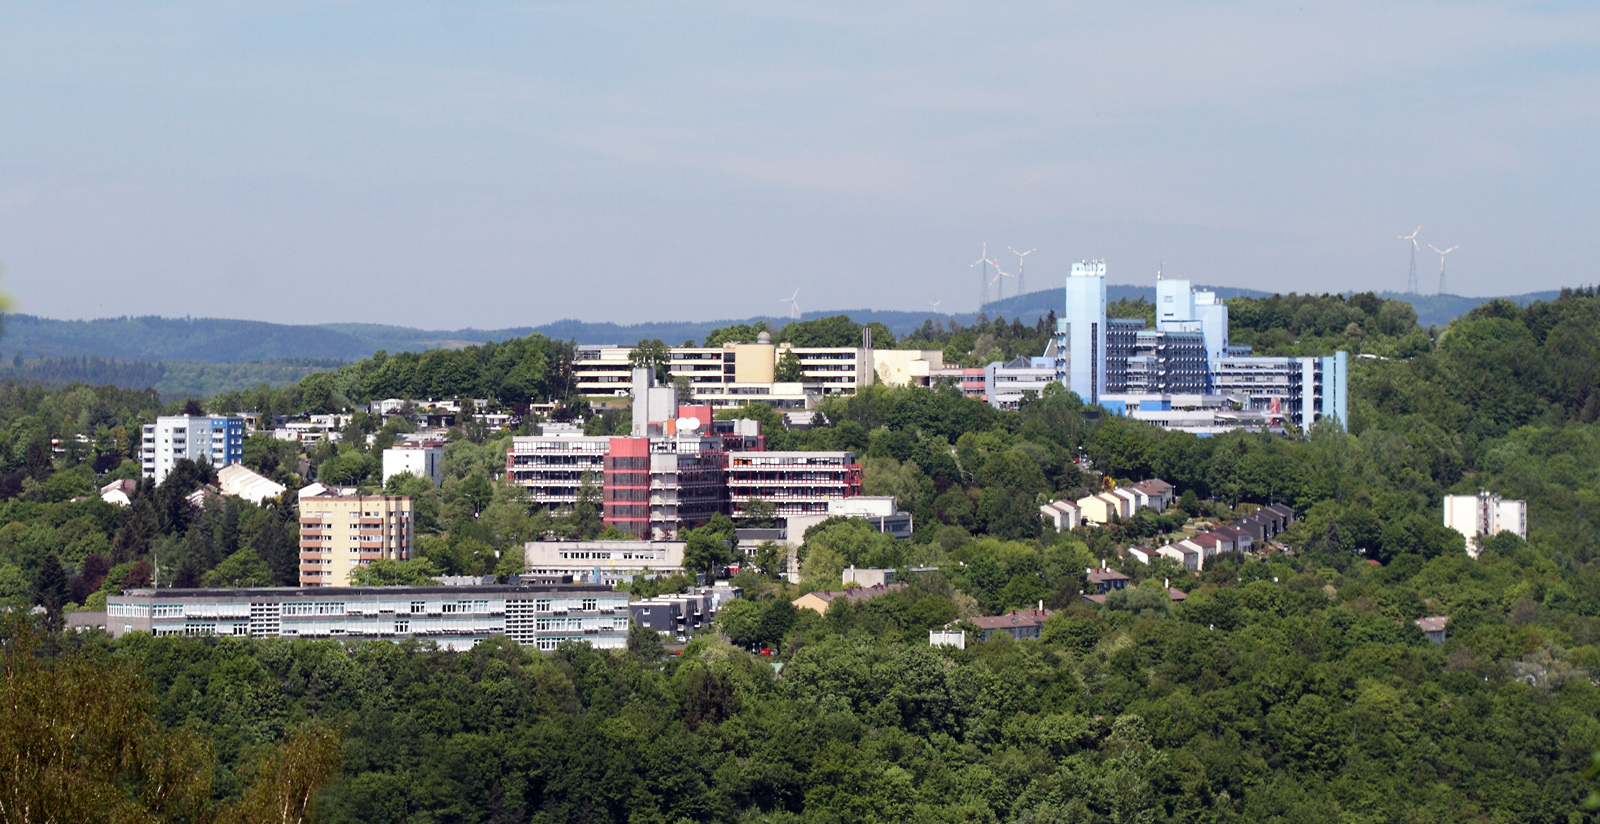
\includegraphics[height=\paperheight,width=\paperwidth]{img/progress.jpg}
}

\begin{document}

\begin{frame}
\titlepage
\end{frame}

\setbeamertemplate{title page}[alternative2]

\titlegraphic{
	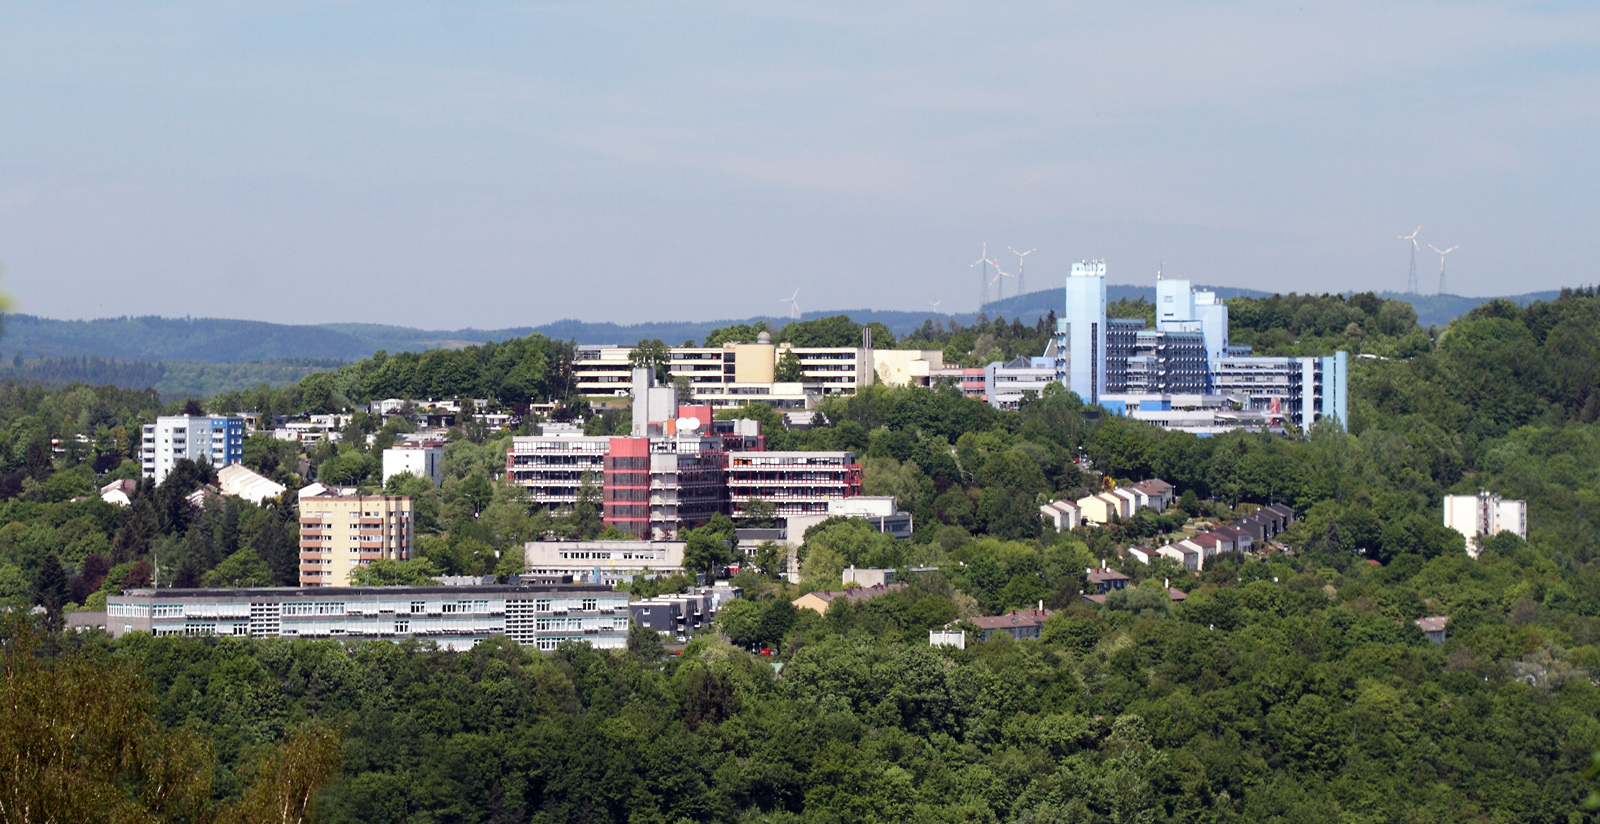
\includegraphics[scale=.32]{img/progress.jpg}
}

\begin{frame}
	\titlepage
\end{frame}

\setbeamertemplate{title page}[alternative3]

\titlegraphic{}

\begin{frame}
	\titlepage
\end{frame}

\setbeamertemplate{title page}[alternative4]

\titlegraphic{
	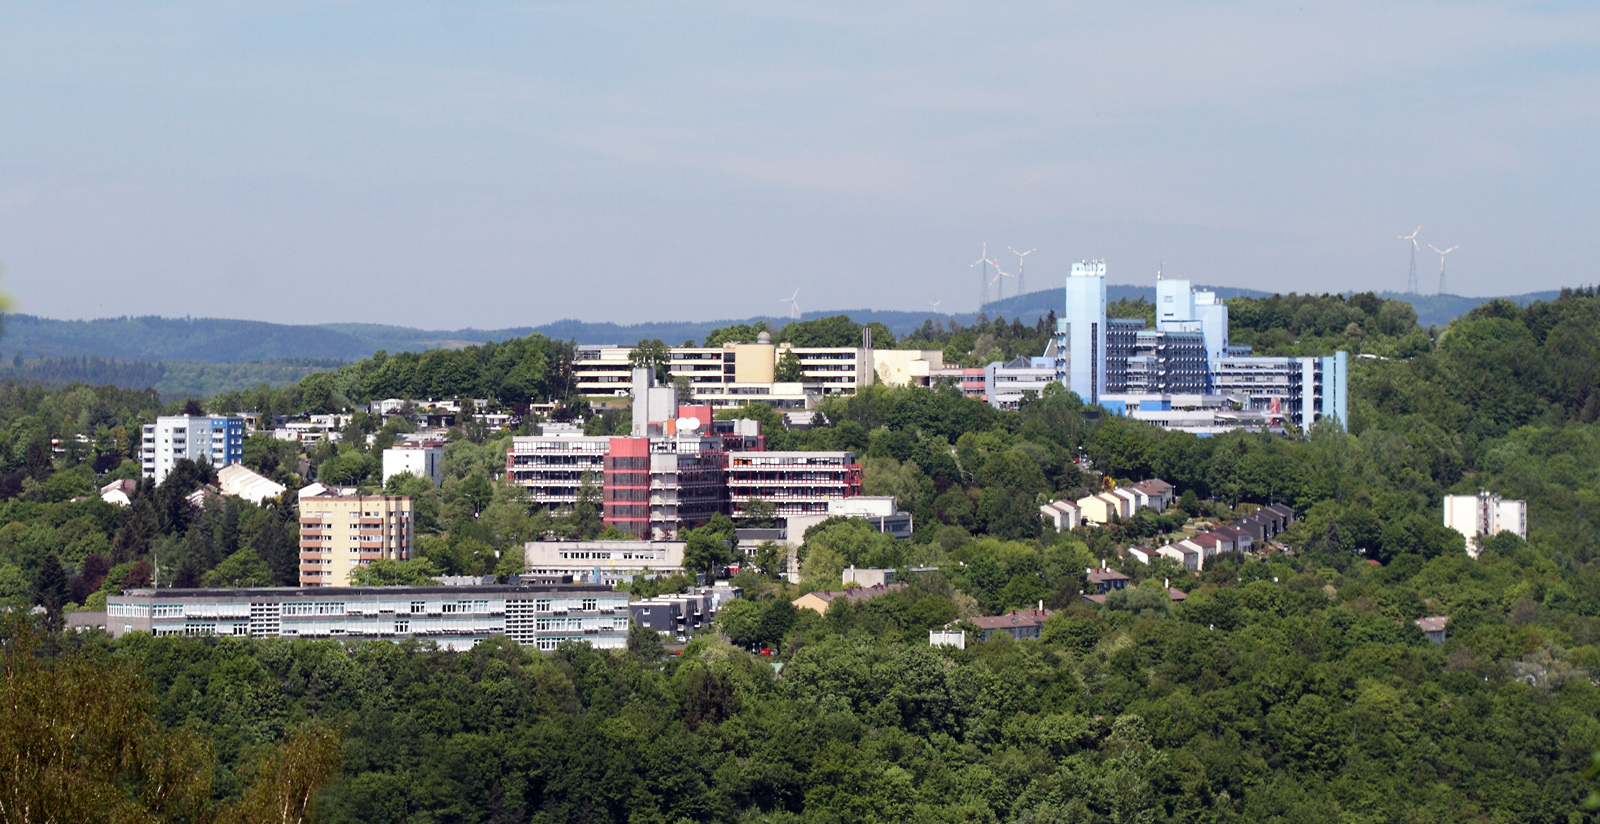
\includegraphics[scale=.32]{img/progress.jpg}
}

\begin{frame}
	\titlepage
\end{frame}

\begin{frame}
	\framesubtitle{A table of contents}
	\tocpage
\end{frame}

\section{Hier steht der Kapitelname}
\subsection{Hier steht der Kapitelname}
\subsection{Hier steht der Kapitelname}
\section{Hier steht der Kapitelname}
\section{Hier steht der Kapitelname}

\begin{frame}{Hier kann eine Überschrift einzeilig\\oder zweizeilig stehen}
	\blindtext
\end{frame}

\begin{frame}{Bildfolie}
	\begin{minipage}{.31\textwidth}
		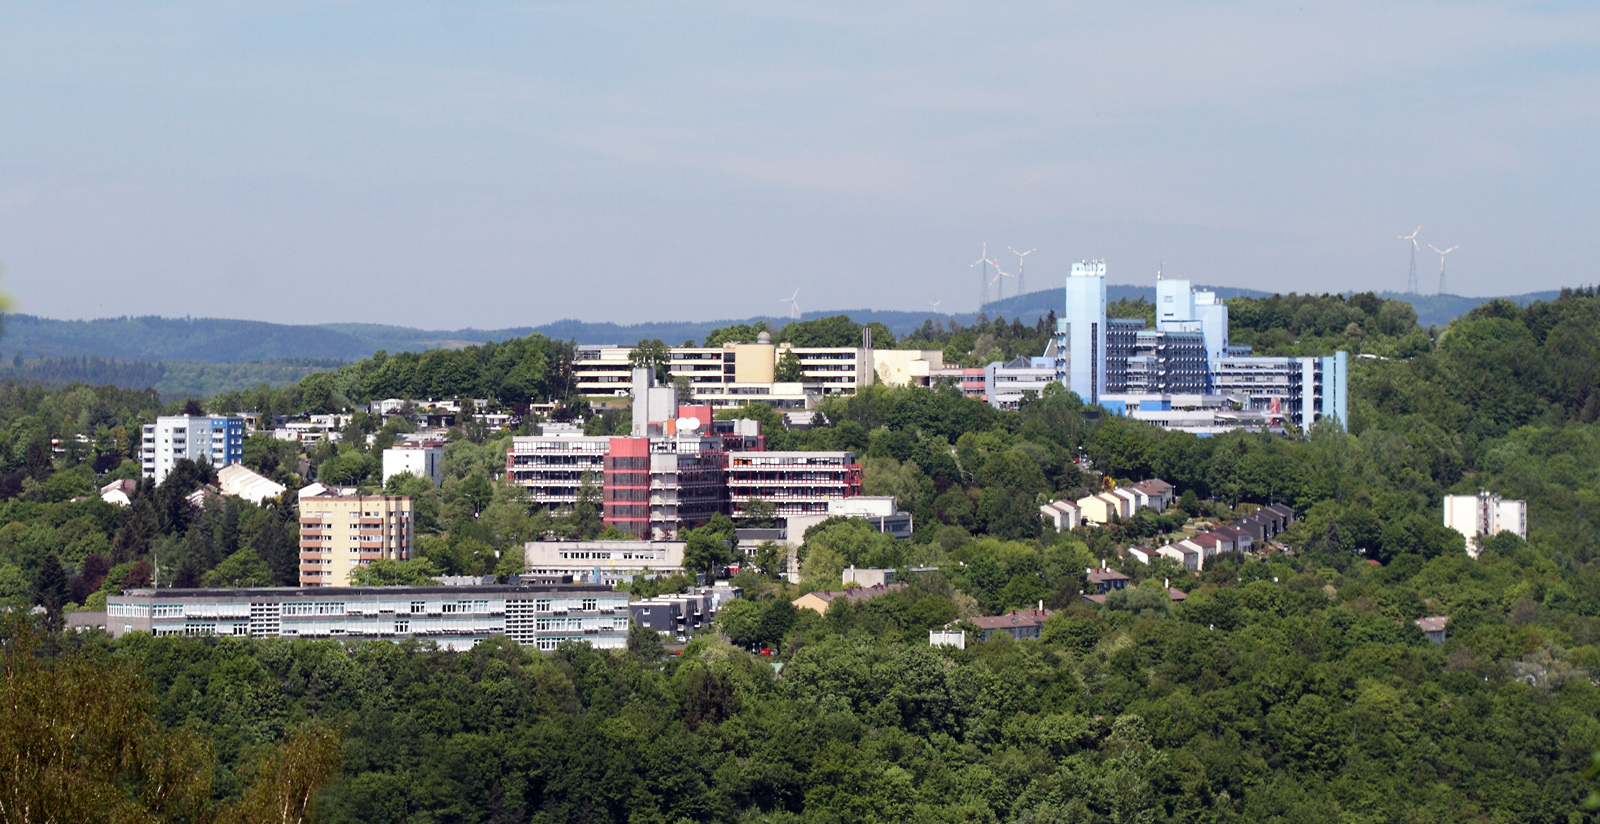
\includegraphics[width=\textwidth]{img/progress.jpg}
		
		\captionof{figure}{Dies ist ein Bild}
	\end{minipage}
	\hfill
	\begin{minipage}{.31\textwidth}
		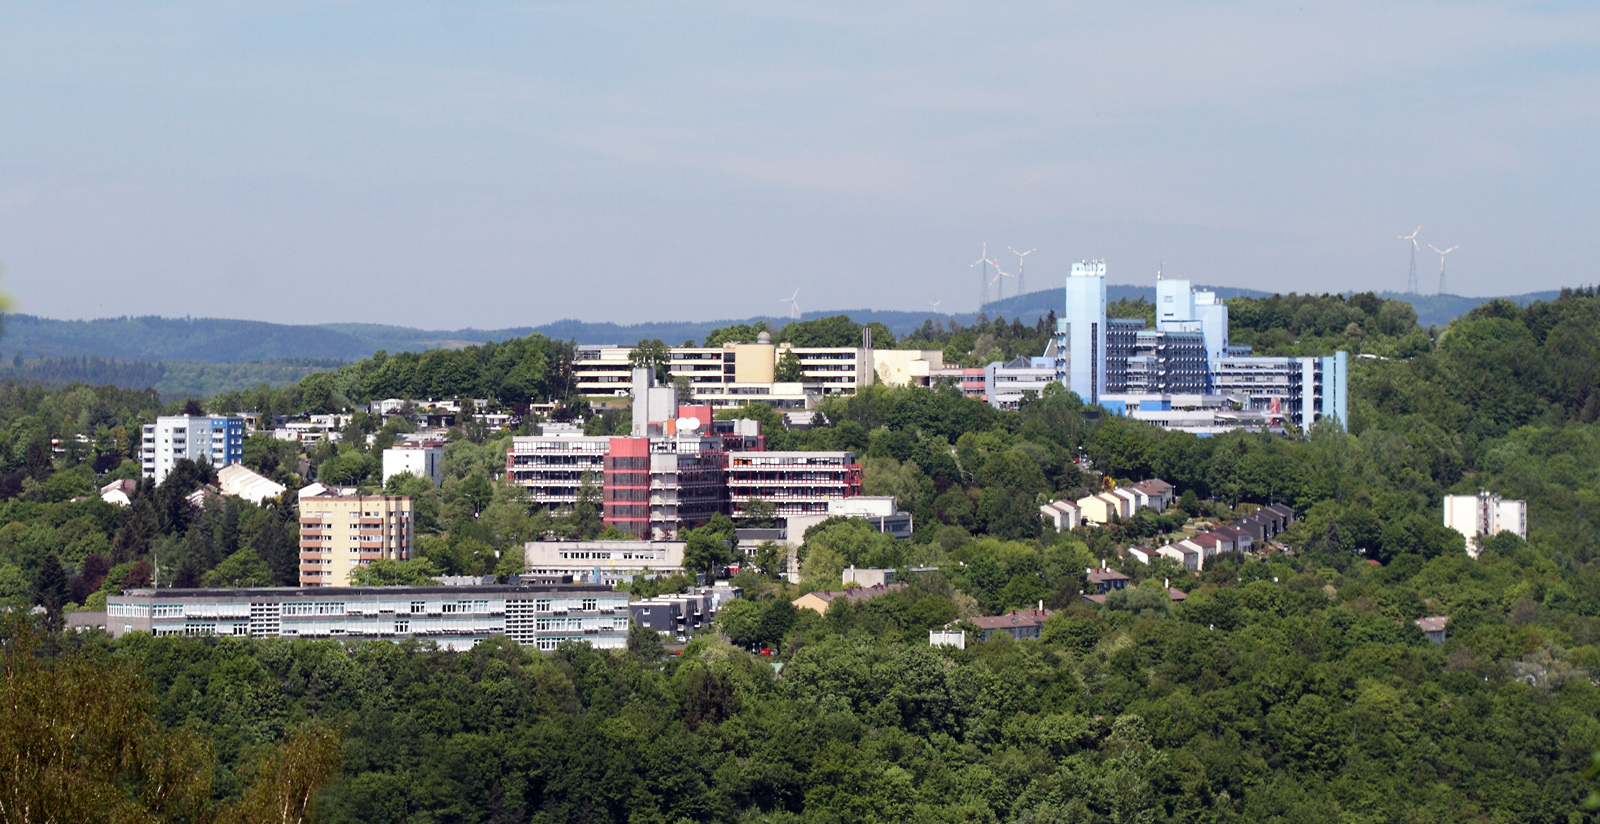
\includegraphics[width=\textwidth]{img/progress.jpg}
		
		\captionof{figure}{Dies ist ein Bild}
	\end{minipage}
	\hfill
	\begin{minipage}{.31\textwidth}
		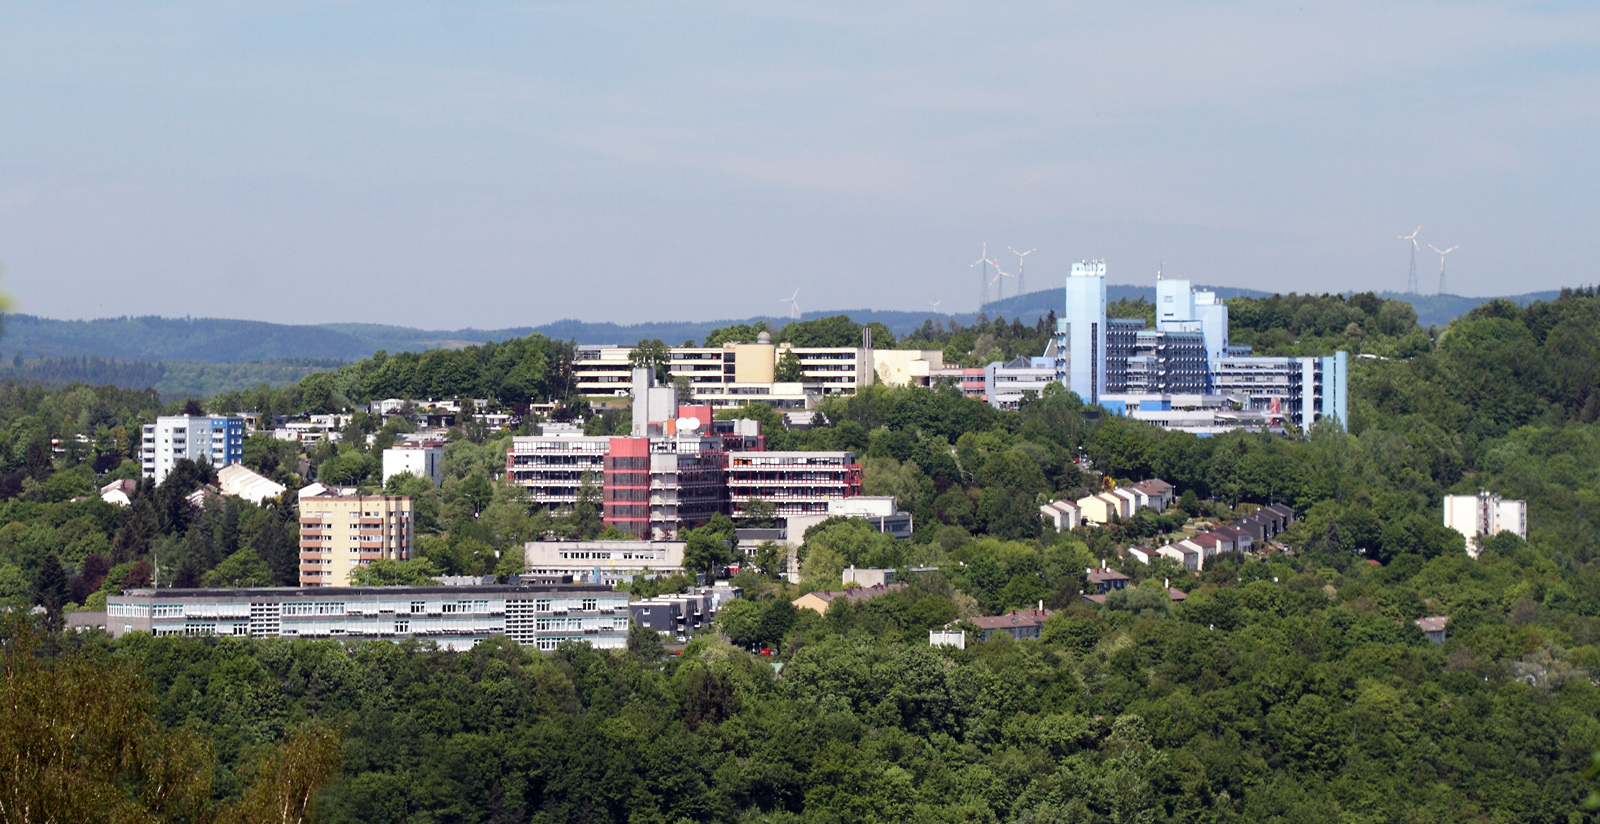
\includegraphics[width=\textwidth]{img/progress.jpg}
		
		\captionof{figure}{Dies ist eine Bildunterschrift, linksbündig gesetzt}
	\end{minipage}
\end{frame}

\begin{frame}{Bildfolie}
	\begin{figure}
		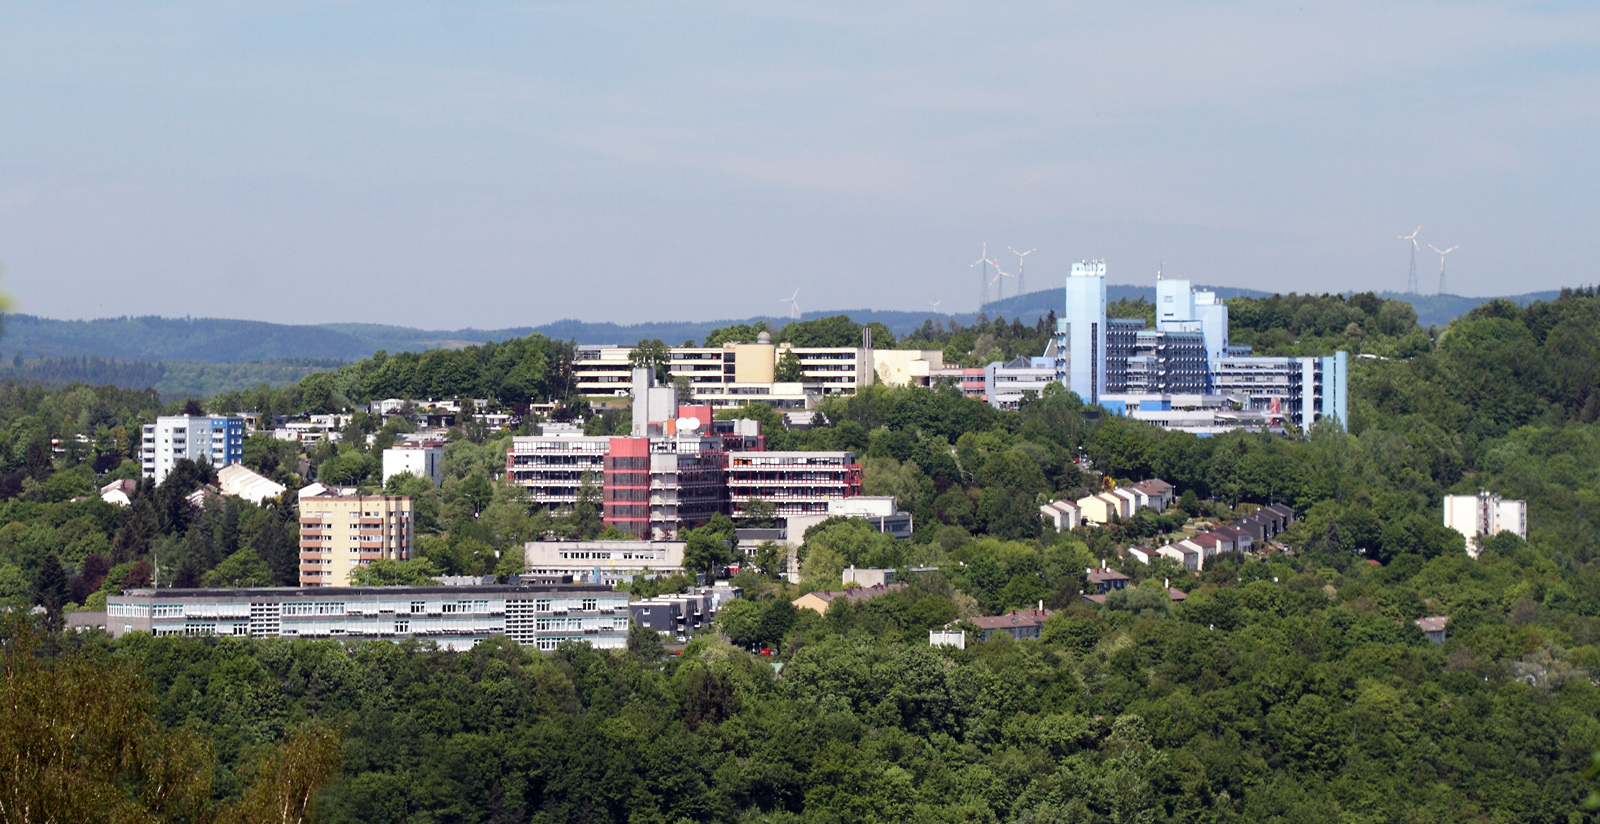
\includegraphics[height=.5\textheight]{img/progress.jpg}
		\caption{Dies ist die Uni}
	\end{figure}
\end{frame}

\begin{frame}{Tabellenfolie}
	\begin{table}
		\begin{tabular}{l | l | l}
			\rowcolor{unigrau}
			
			Spalte 1 & Spalte 2 & Spalte 3\\
		\end{tabular}
	\end{table}
\end{frame}

\end{document}

